
This problem of weak first tokens is pervasive across
relations in LRE. 
\textsc{person\_mother}, 
\textsc{person\_father} and
\textsc{company\_ceo}
are largely evaluated on
first names, many of which occur several times. 
Many archnemeses for
\textsc{superhero\_archnemesis}
also have weak first tokens:
\enote{hs}{check these against the dataset}
``\emph{The} Joker'',
``\emph{Doctor} Doom'',
``\emph{King} Ghidorah''.


\begin{figure}[t]
\centering
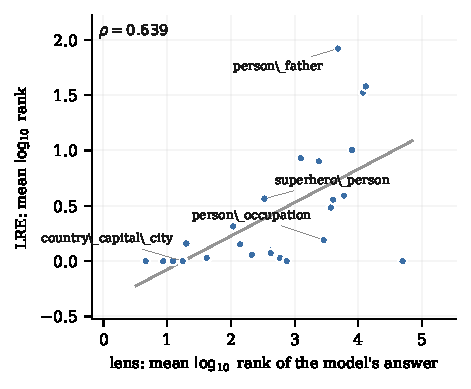
\includegraphics[width=\columnwidth]{fig_rank_rank_mean.pdf}
\caption{The same association, drawn in the coordinate system used for
the per-relation subject-level analysis: the lens's mean $\log_{10}$ rank
of the model's answer against the \emph{LRE's} mean $\log_{10}$ rank of
that same answer, one point per relation. The logarithm is taken per
subject and then averaged, so each subject contributes its order of
magnitude rather than its raw rank. On both axes lower is better, which
is the reverse of Fig.~\ref{fig:main}, whose $x$ axis is negated so that
higher is better. Replacing faithfulness with a rank keeps how far the
LRE was from the model's answer instead of only whether it matched:
Spearman $\rho = 0.639$ as plotted, and $0.699$ using medians rather than
means. Medians are not plotted because any relation with faithfulness
above $0.5$ has a hit as its median subject, which puts 16 of the 25
relations at exactly $0$. Coverage is 25 relations rather than 28:
the two numeric-object relations and
\textsc{person\_band\_lead\_singer} retain too few subjects after
first-token filtering to leave a test set.}
\label{fig:rankrank}
\end{figure}



The subject-level analysis of
\S\ref{sec:subject} requires the two to score the \emph{same} subjects and
uses a single shared split throughout.

The evidence so far is 28 aggregate points, and a skeptic may reasonably
suspect that both measures track some coarse property of a relation rather
than anything about individual entities. Both quantities are, however,
defined per subject: whether the LRE reproduces the model's answer for
that subject, and where the lens ranks it. Asking whether the lens
predicts \emph{which subjects within a relation} the LRE gets right holds
the relation, its prompt, its answer space and its cardinality fixed by
construction -- controlling by design for the covariates
investigated in \S\ref{sec:results}
 -- and converts the claim from a statement about relations
into one about entities, which is what the account asserts.

\paragraph{Design.} The unit is a (relation, subject) pair. The outcome is
whether the LRE's top-1 equals the model's top-1 for that subject; the
predictor is $-\log_{10}$ of the rank at which the lens places that same
token. A relation enters if it has at least 20 scored subjects, a
faithfulness between $0.10$ and $0.90$, and both outcomes present -- a
relation at floor or ceiling has no within-relation variance to predict.
Thirteen relations qualify, giving \textbf{1{,}067 subject-level rows}.
Lens and LRE now take their split from one place and we verify by
fingerprint that they scored identical subjects.

\paragraph{Statistic.} Within each relation we compute the AUC: the
probability that a subject the LRE reproduces has a higher lens score than
one it misses. This is immune to between-relation variation by
construction. We then test whether $\{\mathrm{AUC}_r\}$ lies above $0.5$
with a Wilcoxon signed-rank test across relations. A single pooled
correlation over all 1{,}067 rows would be dominated by between-relation
differences and would re-answer the question of \S\ref{sec:results}.

\begin{table}[t]
\centering\small
\begin{tabular}{@{}lrrrr@{}}
\toprule
relation & $n$ & hits & AUC & $p$ \\
\midrule
superhero\_person & 63 & 35 & 0.835 & 0.000 \\
landmark\_in\_country & 100 & 80 & 0.784 & 0.000 \\
person\_mother & 100 & 11 & 0.766 & 0.004 \\
product\_by\_company & 100 & 68 & 0.715 & 0.001 \\
pokemon\_evolutions & 20 & 5 & 0.707 & 0.197 \\
company\_hq & 100 & 45 & 0.689 & 0.001 \\
company\_ceo & 100 & 12 & 0.688 & 0.035 \\
person\_plays\_position\_in\_sport & 100 & 84 & 0.686 & 0.019 \\
person\_plays\_instrument & 100 & 73 & 0.627 & 0.053 \\
star\_constellation & 100 & 35 & 0.617 & 0.055 \\
person\_occupation & 100 & 66 & 0.494 & 0.922 \\
superhero\_archnemesis & 55 & 18 & 0.467 & 0.700 \\
person\_university & 29 & 10 & 0.268 & 0.046 \\
\midrule
median & 1067 & & \textbf{0.688} & 0.011 \\
\bottomrule
\end{tabular}
\caption{Within-relation discrimination. For each relation, AUC is the
probability that a subject the LRE reproduces has a higher lens score than one
it misses; chance is $0.5$. The final row gives the median AUC and the
Wilcoxon signed-rank test of $\{\mathrm{AUC}_r\}$ against $0.5$.}
\label{tab:subject}
\end{table}


\paragraph{Result.} Median AUC is $\mathbf{0.688}$, above chance for
10 of 13 relations, with Wilcoxon $p = 0.011$ (Table~\ref{tab:subject}).
Permuting outcomes within each relation gives a null median AUC of
$0.500$, matched in $0$ of $2{,}000$ permutations. Scoring all objects
rather than only those whose first token identifies them
(\S\ref{sec:artifact}) gives a median of $0.686$ but $p = 0.084$: the
significant version comes from correcting the scoring, not from dropping
relations.

\paragraph{Is it just confidence?}
\label{par:conf}
If the model is peaked on a subject, both the LRE and the lens may find it
easier, and the association would be real but uninformative. We measure
confidence as the model's top-1 probability at the target position, and
fit a fixed-effects logistic regression stratified by relation, so that
only within-relation variation contributes. Predictors are within-relation
percentile ranks, so a coefficient is the log-odds change across a
relation's own range.

\begin{table}[t]
\centering\small
\begin{tabular}{@{}lrr@{}}
\toprule
model & lens $\beta$ & confidence $\beta$ \\
\midrule
lens only & $+1.90$ & --- \\
lens $+$ top-1 probability & $+1.33$ & $+2.07$ \\
lens $+$ entropy & $+1.42$ & $-1.56$ \\
confidence only & --- & $+2.44$ \\
\bottomrule
\end{tabular}
\caption{The lens effect with and without a control for model confidence.
Coefficients are from a conditional (fixed-effects) logistic regression
of the binary LRE outcome, stratified by relation, on within-relation
percentile ranks of the predictors; $\beta$ is the change in log-odds
across a relation's own range. Significance is by Wald test; all
coefficients have $p < 10^{-4}$.}
\label{tab:conf}
\end{table}

The lens effect survives: an odds ratio of $6.7\times$ across the
within-relation range alone, $3.8\times$ with confidence removed
-- attenuated by 30\%, still at $p < 10^{-4}$. Entropy agrees, with the
expected sign reversal.

But confidence is the \emph{stronger} predictor, at $11.5\times$ alone,
and the two are correlated within relation ($\rho = 0.32$). The honest
statement is therefore that the lens predicts which subjects the LRE
reproduces independently of the model's confidence, that confidence
predicts it better, and that roughly a third of the raw lens effect was
confidence. The asymmetry that makes the lens interesting anyway is that
it is computed without the relation, whereas confidence is measured under
the relation's own prompt.

\paragraph{How large is the effect?} Most of the variation in LRE success
lies \emph{within} relations, not between them: an analysis of variance on
the binary outcome puts $74.7\%$ within and $25.3\%$ between, and the
latent-scale intraclass correlation from a random intercept per relation
agrees at $29.3\%$ between. The subject-level analysis is therefore
addressing the larger component rather than a residual.

It explains a modest share of it. Taking per-relation intercepts as the
baseline, McFadden's pseudo-$R^2$ within relations is $0.047$ for the lens,
$0.075$ for confidence and $0.095$ for the two together. The effect is
real and robust but small, and the bulk of within-relation variation in
LRE success is explained by neither.

\paragraph{The scoring penalizes the lens.} First-token rank scoring
requires the lens to surface the exact answer token, and penalizes it for
producing a synonym or a near neighbor. On a control set of 80 famous
people with a single unambiguous occupation each, the lens places
\textsc{composer} at median rank 3 for composers, but \textsc{writer} at
rank 244 for writers -- whose readings are \emph{novels}, \emph{prose},
\emph{poetry}, \emph{literary}, all correct and none of them the scored
token. The effects we report are therefore lower bounds by an amount we
can demonstrate but not yet quantify.


The fact-level analysis of \S\ref{sec:subject} carries several
caveats of its own. Model confidence predicts LRE success better than
the lens does ($11.5\times$ against $6.7\times$), and explains more of the
within-relation variance ($0.075$ against $0.047$). The lens contributes
independently of it, but neither explains much: together they account for
under a tenth of the within-relation variation in LRE success. Faithfulness there is estimated from a single split per
relation, and a single split is noisy -- one relation scored $0.39$ and
$0.21$ on two draws at identical test-set size -- so the outcome variable
is measured with error that attenuates the association. The thirteen
qualifying relations all sit in the middle of the cardinality range, where
the account is expected to work, making this a fair test of the mechanism
but not of its boundaries. And the inclusion criteria screen on
faithfulness and test-set size, neither of which catches a relation like
\textsc{person\_occupation} where two answers cover 65\% of subjects;
screening on the concentration of the model's answer distribution would
be better, and would have to be fixed in advance.
